% DOCUMENT CLASS %
\documentclass[a4paper, 12pt]{extarticle}   % for A4 Paper, 12pt fontsize and article spacing
\usepackage[left=1.5cm,right=1.5cm,top=2cm,bottom=2cm]{geometry}    % Make the page a little bigger

% PACKAGES%
\usepackage{amsfonts}   % For a basic mathfont (many will be replaced by stix)
\usepackage{amsmath}    % For basic math symbols
\usepackage{bbm}        % For \mathbbm (better version of \mathbb)
\usepackage{mathrsfs}   % For \mathscr
\usepackage{hyperref}   % For footnotes
\usepackage{csquotes}   % For \textquote{}
\usepackage{IEEEtrantools}  % For better alignments
\usepackage{tikz}   % For a macro
\usetikzlibrary{arrows.meta, positioning, calc}	% For protocol diagrams
\usepackage{listings} % For code
\usepackage{xcolor}   % For ... code
\usepackage{microtype}  % For better paragraph formatting
\usepackage{amsthm}   % For custom environments

% FONT CONFIGURATION %
\usepackage[T1]{fontenc}
\usepackage{palatino}

% BASIC SETS %
\newcommand*{\R}{\mathbbm R}    % Set of real numbers
\newcommand*{\N}{\mathbbm N}    % Set of natural numbers (beginning at 0)
\newcommand*{\Z}{\mathbbm Z}    % Set of integers
\newcommand*{\Q}{\mathbbm Q}    % Set of rational numbers

% MACROS %
\newcommand*{\qedbox}{\null\nobreak\hfill\ensuremath{\square}} % Macro for a QED-Box
% for a funny ¯\_(ツ)_/¯-Emoji
\newcommand{\shrug}[1][]{%
    \begin{tikzpicture}[baseline,x=0.8\ht\strutbox,y=0.8\ht\strutbox,line width=0.125ex,#1]
    \def\arm{(-2.5,0.95) to (-2,0.95) (-1.9,1) to (-1.5,0) (-1.35,0) to (-0.8,0)};
    \draw \arm;
    \draw[xscale=-1] \arm;
    \def\headpart{(0.6,0) arc[start angle=-40, end angle=40,x radius=0.6,y radius=0.8]};
    \draw \headpart;
    \draw[xscale=-1] \headpart;
    \def\eye{(-0.075,0.15) .. controls (0.02,0) .. (0.075,-0.15)};
    \draw[shift={(-0.3,0.8)}] \eye;
    \draw[shift={(0,0.85)}] \eye;
    % draw mouth
    \draw (-0.1,0.2) to [out=15,in=-100] (0.4,0.95); 
    \end{tikzpicture}
}

% BASIC CONFIGURATION %
\pagestyle{plain}
\allowdisplaybreaks

% CODE CONFIGURATIONS %
\definecolor{codepurple}{HTML}{7f0055}
\definecolor{comment}{RGB}{0,128,0}
\definecolor{number}{RGB}{9,136,90}
\definecolor{string}{RGB}{163,21,21}

\lstset{
    language=python,
    emph={*, do, od, for, if, fi, then, else, to, def, in, forall, exists},
    firstnumber=1,
    basicstyle=\small\ttfamily,
    breaklines=true,
    breakatwhitespace=false,
    frame=tb,
    captionpos=b,
    %float=t,
    %floatplacement=t,
    abovecaptionskip=0.5cm,
    numbers=left,
    numberstyle=\tiny,
    keywordstyle=\bfseries\color{codepurple},
    emphstyle=\bfseries\color{codepurple},
    mathescape=true,
    keepspaces=true,
    showspaces=false,
    showstringspaces=false,
    showtabs=false,
    stringstyle=\color{string},
    commentstyle=\itshape\color{comment},
    upquote=true,
    texcl=true
}

% EXERCISE ENVIRONMENT %
\theoremstyle{definition}
\newtheorem{exercise}{Exercise}[section]
\setcounter{section}{1} % Don't use \section and this works naturally

% TITLE CONFIGURATION %
\newcommand{\ex}{0}

\title{Data Visualization \\ \small Exercise Sheet \ex}
\date{Winter Term 2025/26}
\author{
    Henri Heyden \\%
    \small stu240825%
    \and
    Julia Schröder \\%
    \small stu252018%
    \and
    Rebecca Ziebell \\%
    \small stu250567%
}


\renewcommand{\ex}{4}
\setcounter{section}{\ex}

\begin{document}
    \maketitle

    \begin{exercise}[Colors]
        I prefer the second color scheme over the others, as they have individual problems.

        The most obvious point is, that the viewer may interpret a link between \emph{Men over 60} and \emph{Women under 20}---the gradient implies continuity between groups!
        This problem does not appear in the second nor the third color scheme.
        Regarding the third color scheme, there are some additional problems to consider.
        
        Firstly, the gradients are chosen as such, that the younger men and women are not as easily seen on paper, as the older participants of the study.
        This could be interpreted as a false proportionality between age and importance to the information conveyed in the graphic.
        Secondly, there is not a big difference in between the colors inside the male and respectively female groups, which may subjugate the viewer to not perceive a difference between the subgroups in some graph charts, e.g., a multiline chart or scatter plot.
        This problem could be mitigated by choosing a more fitting chart type, e.g., a bar chart or radial tree.

        Lastly, the second color scheme offers some simplicity, which the third color scheme does not have: The individual count of different subgroups is smaller---enabling to use more contrasting colors for each subgroup.
        This is also an important point regarding the \emph{purpose} of the chart---it is supposed to highlight differences between older and younger people.
        Depending on the information to convey, the designer may benefit from using a small color scheme.
    \end{exercise}

    \begin{exercise}[Likert Scale] \hfill
        \begin{enumerate}
            \item This question matches best to the second color scheme.
        \end{enumerate}
    \end{exercise}

    \begin{exercise}[Less Color]
        This visualization looks somewhat pretty because of the many colors used, but it isnt functional at all.
        It isnt easy to gather much information out of this graph. To fix this problem you could group some of the categories if possible.
        You could also, instead of using many different colors, use diffrent fonds of grey or choose one color and use different luminance levels.
        For example blue. (light blue, blue, dark blue, etc.). Dont use too vivid colors, because they compete for attention and make it hard to focus on the data.
        Also, colors should not be the only distinguishing feature. You could use aspects like line thickness, transparency and labels to make the visualization
        nicer to look at.

    \end{exercise}

    \begin{exercise}[Color Vision Deficiency Pt. 1]
    \end{exercise}

    \begin{exercise}[Color Vision Deficiency Pt. 2]
        By putting the visualization into the color-blindness-simulator, it gets noticable that people who suffer from
        Protanopia (red blindness), Deuteranopia (green blindness), Protanomaly (red weakness), Deuteranomaly (green weakness) and Monochromacy
        really struggle to distinguish between the two bars. 
        By changing the colors of the bars, everyone who has a color vision deficieny can still see and use the information on this chart.

        \begin{center}
                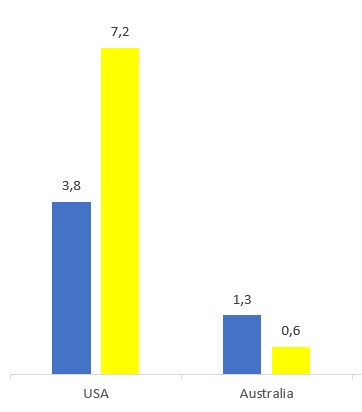
\includegraphics[width=0.5\textwidth]{barchart.png}
        \end{center}

    \end{exercise}
    
    \setcounter{exercise}{6}
    \begin{exercise}[Color Pallets -- Dataset Handling]
    \end{exercise}
\end{document}
